% !TeX root = ../../tesi.tex

DEIMv2 was considered the most direct candidate for this thesis because it explicitly targets the same design space of interest: high-accuracy \emph{real-time} object detection under practical computational constraints \cite{huang_real-time_2026}. Architecturally, DEIMv2 extends the RT-DETR family by combining an end-to-end transformer-based detector with \textbf{stronger backbone features}. 
It offers many variants that span a wide range of model sizes and computational budgets, making it a versatile choice for comparative evaluation. Specifically:
\begin{itemize}
    \item For the mainstream variants (S, M, L, X), it adopts \textbf{DINOv3-pretrained} or distilled Vision Transformer backbones and introduces a \textbf{\emph{Spatial Tuning Adapter} (STA)} to transform the single-scale ViT output into multi-scale features suitable for detection. 

    \item For the ultra-lightweight variants (atto, femto, pico, nano), it instead relies on pruned \textbf{HGNetv2} backbones, thereby covering GPU, edge, and mobile deployment scenarios within the same design family \cite{huang_real-time_2026}.
\end{itemize}
\begin{figure}[h]
    \centering
    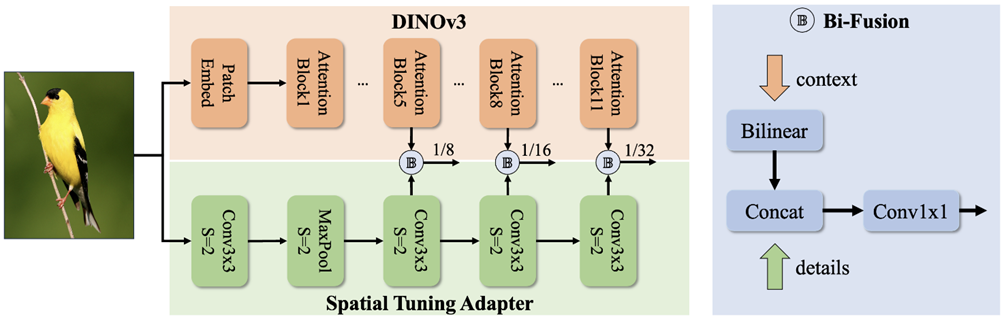
\includegraphics[width=0.8\textwidth]{images/DEIMv2.png}
    \caption{DEIMv2 architecture overview, illustrating the use of DINOv3 backbones and the Spatial Tuning Adapter (STA) to produce multi-scale features for detection \cite{huang_real-time_2026}.}
    \label{fig:DEIMv2_architecture}
\end{figure}

From the perspective of the present application, the main strength of DEIMv2 lies in its ability to combine rich semantic representations with fine-grained local details by integrating DINOv3-based features into an RT-DETR-derived detection framework. This aspect is particularly attractive for the inspection tasks considered in the thesis, since the relevant visual cues may include both global shape information and localized appearance variations. Moreover, DEIMv2 preserves the end-to-end advantages inherited from RT-DETR, including NMS-free prediction, while improving the performance--cost trade-off through stronger features, a simplified decoder, and improved training strategies such as Copy-Blend augmentation \cite{huang_real-time_2026}. The model is also highly scalable: the paper reports strong performance not only for the largest variants, but also for compact versions designed for resource-constrained deployment.
\begin{figure}[h]
    \centering
    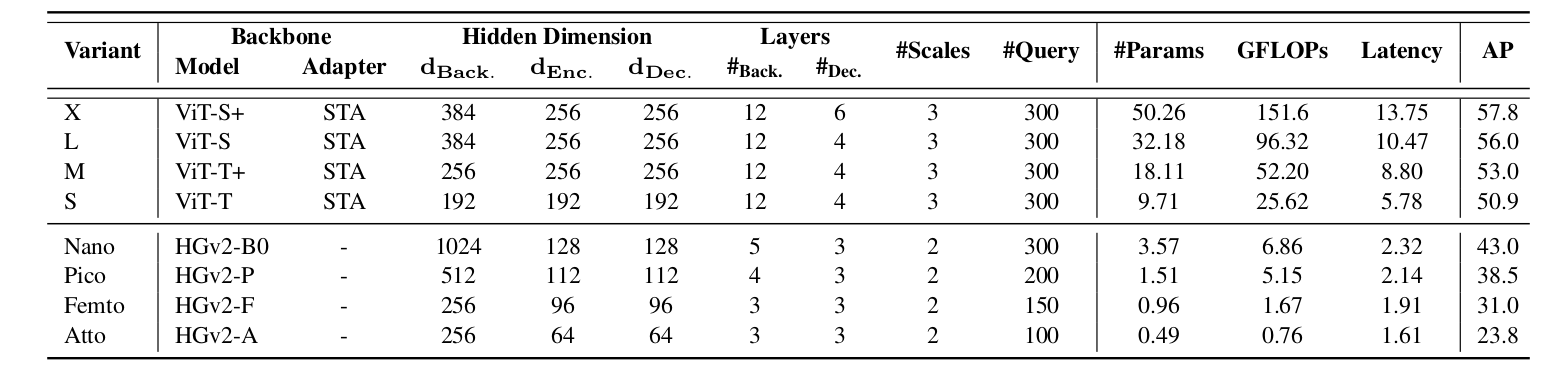
\includegraphics[width=0.9\textwidth]{images/DEIM_results.png}
    \caption{Summary of DEIMv2 results across model scales, highlighting the balance between detection accuracy, latency, and parameter efficiency \cite{huang_real-time_2026}.}
    \label{fig:DEIMv2_results}
\end{figure}

The main limitation of DEIMv2 is that part of its performance advantage depends on the availability of powerful pretrained backbones, especially for the larger variants. In other words, the strongest configurations benefit from large-scale representation learning prior to the downstream detection task. Even so, the model remains particularly compelling within the present comparative study because it combines strong reported accuracy, broad scalability, and clear compatibility with real-time detection requirements \cite{huang_real-time_2026,zhao_detrs_2024}.
